The key to understand this solution is to see from another point of view the atmospheric drag phenomena. Once we have designed the constellation to provide certain coverage to specific points of the globe, the action of increasing the height of the orbit has the effect of increasing the footprint area on the surface of the earth. As the constellation is set, the time that take the satellites to reach the design height is extra lifetime. 

From this point of view, the atmospheric drag phenomena can be recomputed and plotted it in this new way:

\begin{figure}[H]
\centering
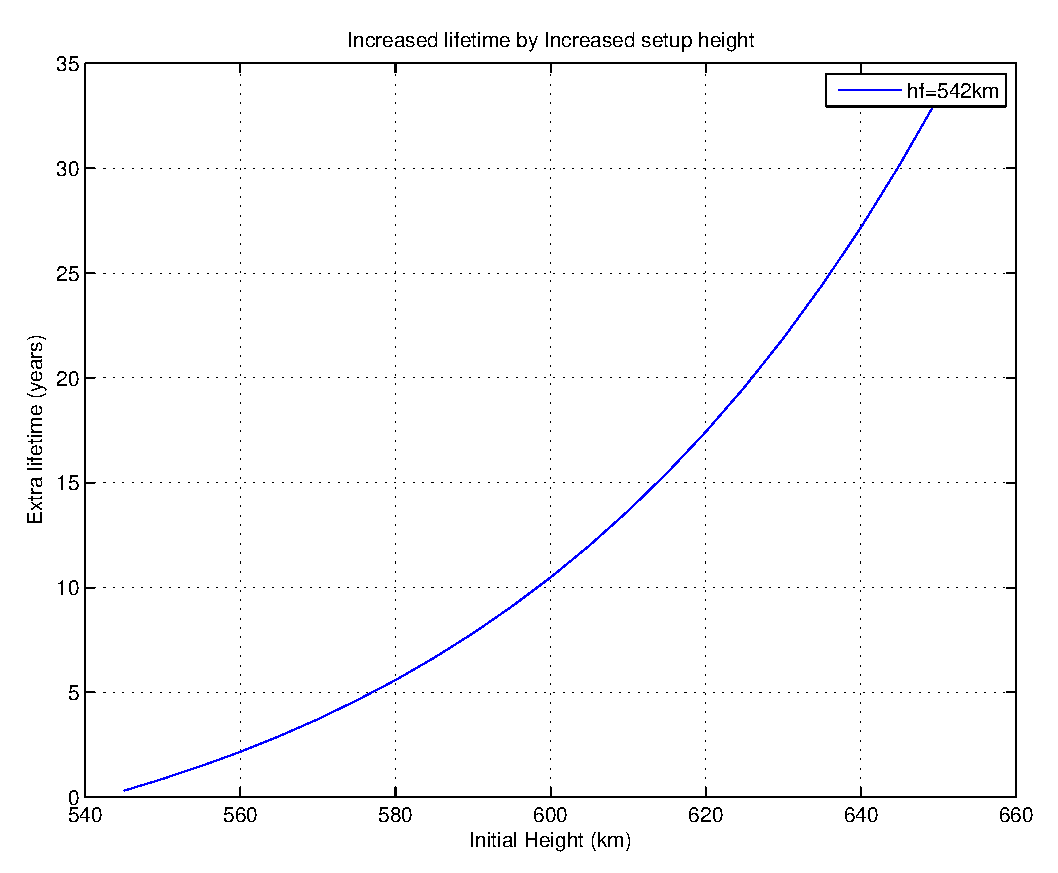
\includegraphics[scale=0.7]{ExtraLifetime/ExtraLifetime.eps}
\caption{Increase in the Lifetime obtained by setting the constellation in a higher orbit}
\end{figure}

As it can be seen, the lifetime increases radically with time. However, this is a dangerous solution, since the coupling with another design parameters is compromised. To list the complications that can lead to:

\begin{itemize}
\item \textbf{Clients: }With the current technology, the satellites currently in orbit are set to point towards Earth. This means, if the contellation's satellites are at a higher orbit, the contact is impossible. As the market study reveals, it is important to place the satellites as low as possible.
\item \textbf{Spacecraft Subsystems: }A higher orbit means a higher gain for the antennas and therefore an increase in the required power.
\item \textbf{Constellation Reconfiguration: } The overall time to reconfigurate the constellation increases with height, since the period of the transition orbits is higher.
\end{itemize}

\textbf{In conclusion\\}
This tool is a very powerful option to deal with the orbit decay, even though it is not exactly an operation of Station Keeping itself. Given the high correlation it shows with another subsystems, the possibility of using it needs to be considered while the other design decisions are taken.